\documentclass[pagesize=auto]{scrartcl}

\usepackage{fixltx2e}
\usepackage{etex}
\usepackage{lmodern}
\usepackage[T1]{fontenc}
\usepackage{textcomp}
\usepackage[svgnames]{xcolor}
\usepackage{tikz}
\usepackage{amsmath}
\usepackage{mathtools}
\usepackage{booktabs}
\usepackage{listings}
\usepackage{microtype}
\usepackage{hyperref}

\newcommand*{\mail}[1]{\href{mailto:#1}{\texttt{#1}}}
\newcommand*{\pkg}[1]{\textsf{#1}}
\newcommand*{\cs}[1]{\texttt{\textbackslash#1}}
\makeatletter
\newcommand*{\cmd}[1]{\cs{\expandafter\@gobble\string#1}}
\makeatother
\newcommand*{\opt}[1]{\texttt{#1}}

\addtokomafont{title}{\rmfamily}

\lstset{%
  language=[LaTeX]TeX,%
  columns=flexible,%
  upquote=true,%
  numbers=left,%
  basicstyle=\ttfamily,%
  keywordstyle=\color{Navy},%
  commentstyle=\color{DimGray},%
  stringstyle=\color{SeaGreen},%
  numberstyle=\scriptsize\color{SlateGray}%
}

\title{The \pkg{type1cm} package for \LaTeX\thanks{This manual corresponds to \pkg{type1cm.sty}~v0.04, dated~2002/09/05.}}
\author{David Carlisle\thanks{\mail{david@dcarlisle.demon.co.uk}}}
\date{2002/09/05}


\begin{document}

\maketitle

\noindent
\LaTeX\ separates its internal notion of font specification
from the external fonts available on the system by means of
`Font Shape Specifications', that are normally held in 
`Font Descriptor' (\textsc{fd}) files.

The \textsc{fd} files that come with \LaTeX\ that refer to the standard
Computer Modern set (and the related \AmS\ set) are based on
the classical bitmap fonts which are available in `magstep'
sizes only. For instance The specification of the main roman font is
%
\begin{lstlisting}
\DeclareFontShape{OT1}{cmr}{m}{n}
 {  <5> <6> <7> <8> <9> <10> <12> gen * cmr
    <10.95> cmr10
    <14.4>  cmr12
    <17.28><20.74><24.88>cmr17}{}
\end{lstlisting}
%
which says for instance that no font is available at 10.5\,pt (\LaTeX\ %
will substitute the nearest available size if you ask for this)
and similarly the font is not available at all above 25\,pt.

Such restrictions are essential with bitmap fonts to save generating
huge numbers of bitmaps for any size that might be requested, however
with scalable versions of the fonts these restrictions are not really 
needed. For instance the equivalent definition defined here is:
%
\begin{lstlisting}
\DeclareFontShape{OT1}{cmr}{m}{n}{
        <-6>    cmr5
        <6-7>   cmr6
        <7-8>   cmr7
        <8-9>   cmr8
        <9-10>  cmr9
        <10-12> cmr10
        <12-17> cmr12
        <17->   cmr17
      }{}
\end{lstlisting}
%
which means that you can (Although some may consider it bad style)
go
%
\begin{verbatim}
\fontsize{10.7pt}{12pt}\selectfont
\end{verbatim}
%
and be given a suitably scaled
version of \texttt{cmr10} and a baseline setting of 12\,pt. Similarly if you really
want, you can go
%
\begin{verbatim}
\fontsize{2cm}{2.5cm}\selectfont
\end{verbatim}
%
and use \texttt{cmr17} scaled
to 2\,cm height for a special display context.

\begin{flushleft}
  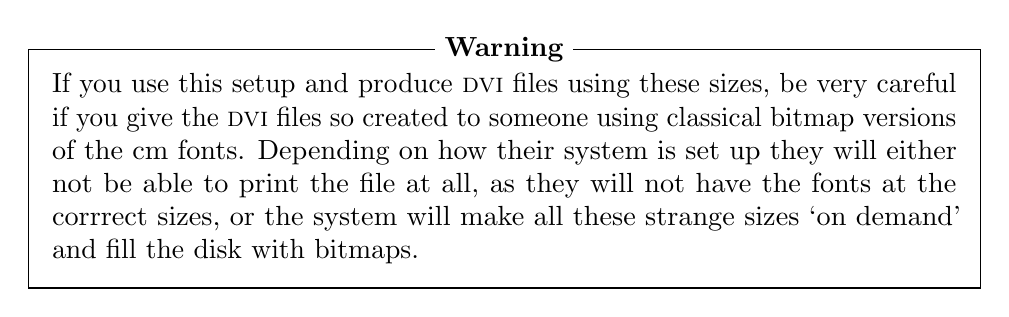
\begin{tikzpicture}
    \node[draw=black, inner sep=2ex] (frame) {%
      \parbox{\dimexpr\linewidth-4ex-1pt\relax}{%
        If you use this setup and produce \textsc{dvi} files using these sizes, be very
        careful if you give the \textsc{dvi} files so created to someone using classical
        bitmap versions of the cm fonts. Depending on how their system is set up
        they will either not be able to print the file at all, as they will not
        have the fonts at the corrrect sizes, or the system will make all these
        strange sizes `on demand' and fill the disk with bitmaps.
      }%
    };
    \node[fill=white] at (frame.north) {\textbf{Warning}};
  \end{tikzpicture}
\end{flushleft}

So the default way of using this package is as a \LaTeX\ package file.
Install \texttt{type1cm.sty} as described below and then just add
%
\begin{verbatim}
\usepackage{type1cm}
\end{verbatim}
%
to your document. This will override the definitions for all the fonts
and so the standard \textsc{fd} files are not used.
The disadvantage of this method is all the definitions are then loaded
into memory, even for fonts you don't use in the document. (However
only the size specifications are so loaded, not the fonts themselves).
However the advantage is that you can always choose not to specify 
\verb|\usepackage{type1cm}| and so use the same font sizes (and get the
same line and page breaks) as everyone else.

Alternatively you may use this package to produce a set of fd
files that \emph{replace} the standard files (such as \texttt{ot1cmr.fd})
You will then need to remake the \LaTeX\ format by running \texttt{initex} on
\texttt{latex.ltx} (as some \textsc{fd} files are loaded into the format). Then you
will not need to use \cmd{\usepackage}. All your documents will have the
freedom of scalable font choices.


\section{Installation instructions}

\renewcommand*{\labelenumi}{\theenumi)}

The installation is controlled by the file \texttt{type1cm.ins} which you may
edit in two places.
%
\begin{enumerate}
\item If you have not got the \AmS\ Font set available in scalable form
  remove the `\verb|%|' from the line \verb|%\def\ams{}|\\
  This will cause a more restricted font specification to be used.

  If you have an extended \AmS\ font set available in scalable form
  (\textsf{msam6}, \textsf{msam8} and \texttt{msam9} in addition to \textsf{msam5}, \textsf{msam7} and \textsf{msam10})
  then remove the `\verb|%|' from the line \verb|%\def\ams{ams,extra}|

\item If after reading the warning above you decide to make a set of fd 
  files, remove the `\verb|%|' from the line \verb|%\makefdtrue|
\end{enumerate}

Then run \texttt{tex} (or \texttt{latex}) on the file \texttt{type1cm.ins} and a package file
\texttt{type1cm.sty} (and perhaps a set of \textsc{fd} files) will be produced
which you should place in a directory where \TeX\ looks for input files.


\section{Small technical note about the Font Shape specifications used.}

I consistantly specified that given a requested size, the largest
available font size smaller than the requested size should be used
and then enlarged to the requested size. The exception being sizes
smaller than the smallest available font, which use a reduced version
of that font. The rationale for this is that enlarging a small font
typically produces a rather `fat' font, but something readable, whereas
shrinking a font may produce something unreadable quite quickly

So for \textsf{msam} (if `\opt{extra}' is not specified) I used:
%
\begin{lstlisting}
\DeclareFontShape{U}{msa}{m}{n}{
        <-7>    msam5 
        <7-10>  msam7
        <10->   msam10
        }{}
\end{lstlisting}
%
That is sizes strictly below 7\,pt use \textsf{msam5}, 7\,pt to (less than) 10\,pt
use \textsf{msam7} and sizes 10\,pt and above use \textsf{msam10}.

This differs from the Specification that the \AmS\ use for the scalable
\AmS\ fonts (used by the \opt{psfonts} option to the \pkg{amsfonts} package)
They use
%
\begin{lstlisting}
\DeclareFontShape{U}{msa}{m}{n}{
       <-6>      msam5 
       <6-8>     msam7 
       <8->      msam10
  }{}
\end{lstlisting}
%
This has the advantage of minimising the scaling used, so for instance
a 9\,pt request is satisfied by \textsf{msam7} scaled up to~9 by this package, but
by \textsf{msam10} scaled down to~9 by the \AmS\ package.

In practice this is not likely to make a difference that anyone notices,
but it could in principle affect line breaks etc, so I thought that
I would mention it here.

\clearpage


\section{History}

\begin{description}
\item[1997/01/27 v0.02 BlueSky/Y\&Y Type1 CM font definitions (DPC)] \leavevmode \\
  Possibly first public release? Maybe there was a 0.01..

\item[2002/04/01 v0.03 BlueSky/Y\&Y Type1 CM font definitions (DPC)] \leavevmode \\
  \textsf{cmdunhill} hasn't worked since the beginning: \cmd{\hyp\clap{\raisebox{-1.9ex}{\rmfamily\textuparrow}}enchar}

  Reported by Brian Mays via the Debian bug tracking system.
  Also, made distribution conditions LPPL (previously unspecified)
\end{description}

\end{document}
